% !TeX spellcheck = cs_CZ
%{\tikzset{external/prefix={tikz/FYZII/}}
% \tikzset{external/figure name/.add={ch02_}{}}
%---------------------------------------------------------------------------------------------------
% file fey1ch01_02_03.tex
%---------------------------------------------------------------------------------------------------
% ==================== Kapitola: Diferenciální počet vektorových polí ==============================
\setchaptertoc
\chapter{Diferenciální počet vektorových polí}\label{fyz:IIchapII}


  \section{Chápání fyziky}
    Fyzik potřebuje mít schopnost zkoumat problémy z několika hledisek. Exaktní analýza reálných
    fyzikálních problémů je obvykle velmi složitá. Jakákoliv konkrétní fyzikální situace se může
    ukázat příliš spletitou na to, aby bylo možné ji analyzovat přímo řešením diferenciální rovnice.
    Přesto lze získat velmi dobrou představu o chování systému, má-li fyzik určitou schopnost
    vycítit charakter řešení v různých situacích. Přitom jsou velice prospěšné takové představy jako
    siločáry, kapacita, odpor a indukce. Proto strávíme mnoho času při jejich analýze. Tím získáme
    cit pro to, co se v různých situacích děje. Na straně druhé ani jeden z heuristických modelů,
    takových, jako jsou siločáry, není adekvátní skutečnosti a přesný ve všech situacích. Existuje
    pouze jediný způsob formulace zákonů, a to pomocí diferenciálních rovnic. Předností rovnic je
    jejich fundamentálnost, a pokud je nám známo, i přesnost. Jestliže jste se naučili diferenciální
    rovnice, vždy se k nim můžete vrátit. Neexistuje přitom nic, co by bylo třeba se odnaučit.
    
    Pochopit, co se v různých situacích děje, nám zabere určitý čas. Budeme muset řešit rovnice. 
    Pokaždé, když řešíme rovnice, se něco dozvíme o charakteru řešení. Aby jsme si tato řešení 
    zapamatovali, bude také užitečné zkoumat, co znamenají z hlediska siločar a dalších pojmů. To 
    je cesta, kterou rovnicím opravdu „porozumíme“. V tom je rozdíl mezi matematikou a fyzikou. 
    
    Co opravdu znamená pochopit rovnici, tj. více než ve stri\-ktně matematickém smyslu, vyjádřil 
    Dirac. Řekl: \emph{„Rozumím tomu, co rovnice znamená, umím-li určit vlastnosti jejího řešení, 
    aniž bych ji ve skutečnosti řešil.“} Ovládáme-li tedy způsob, jak se dovědět, co se děje v 
    daných  situacích, aniž bychom rovnice skutečně řešili, „chápeme“ rovnice v aplikaci na tyto 
    situace. Fyzikální chápání je naprosto nematematické, nepřesné a neexaktní, ale pro fyzika 
    naprosto nevyhnutelné.
    
    \luagraphic[0.9]{fyz_fig030.pdf}{Určení směru vektoru $\vec{A}\times\vec{B}$ pomocí 
    pravotočivého šroubu}{fyz:fig030}

    Kurz, jako je tento, bývá obvykle založen na postupném budování fyzikálních představ - začíná 
    jednoduchými situacemi a pokračuje situacemi stále složitějšími. Vyžaduje to, abychom neustále 
    zapomínali věci, které jsme se naučili dříve - věci, jež platí v určitých situacích, ale 
    neplatí obecně. Například „zákon“, že elektrická síla se mění s druhou mocninou vzdálenosti, 
    neplatí vždy. My dáváme přednost opačnému postupu. Raději napřed probereme úplné zákony a pak 
    budeme postupovat zpět a aplikovat je na jednotlivé situace, se souběžným rozvíjením 
    fyzikálních představ. A to je to, co se chystáme dělat nyní.
    
    Náš přístup je úplným opakem historického přístupu, při němž se předmět podává na základě 
    experimentů, které o něm poskytly informaci. Předmět fyziky však budovalo velmi mnoho bystrých 
    lidí během uplynulých více než 200 let, a protože my máme na nabytí informací jen omezenou 
    dobu, není v našich silách probrat vše, co udělali oni. Bohužel, jedno z toho, co přitom bude 
    zřejmě chybět v těchto přednáškách, je historický, experimentální postup. Je naděje, že je 
    možné nahradit tento nedostatek v určité míře laboratorními cvičeními. Vše, co musíme pustit ze 
    zřetele, lze také doplnit čtením encyklopedií, v nichž se občas vyskytují historické 
    články o elektřině a o jiných oblastech fyziky. Historickou informaci najdeme také v mnoha 
    učebnicích elektřiny a magnetizmu.
    
  %----------------------- Vektorový počet ---------------------------------------------------------
  \section{Vektorový počet}
    Nyní začněme s abstraktním, matematickým pohledem na teorii elektřiny a magnetizmu. Základní 
    myšlenkou je vysvětlit význam zákonů formulovaných v kapitole \ref{fyz:IIchapI}. Ale abychom 
    to udělali, musíme nejdříve vysvětlit novou a zvláštní symboliku, kterou chceme použít. Takže 
    na chvíli zapomeňme na elektromagnetizmus a věnujme se matematice vektorových polí. Je velmi 
    důležitá nejen pro elektromagnetizmus, ale pro všechny druhy fyzikálních situací. Diferenciální 
    počet vektorů je pro všechna odvětví fyziky stejně důležitý jako obyčejný diferenciální a 
    integrální počet. Tak se do toho pusťme.

    Dále uveďme několik faktů z vektorové algebry, přičemž předpokládáme, že je již známe: V 
    pravoúhlém kartézském systému je každý bod prostoru určen polohovým vektorem $\vec{r}$, který 
    má složky $x,\,y,\,z$, což budeme zapisovat takto:
    \begin{equation}\label{fyz:eq688}
      \vec{r}\equiv(x,y,z)=\vec{i}x+\vec{j}y+\vec{k}z
    \end{equation}
    kde $\vec{i},\,\vec{j},\,\vec{k}$ jsou jednotkové vektory ve směru osy $x,\,y,\,z$. Velikost 
    vektoru $\vec{r}$ určíme ze vztahu
    \begin{equation}\label{fyz:eq689}
      \abs{\vec{r}}\equiv r = \sqrt{x^2+y^2+z^2}
    \end{equation}
    Pro osvěžení pár faktů z vektorové algebry pro vektory$\vec{A},\,\vec{B},\,\vec{C}$ uveďme 
    následující vztahy: 
    \begin{equation*}
      \vec{A}\cdot \vec{B}\cdots\text{skalár} \quad\quad                        
      \vec{A}\times\vec{B}\cdots \mathrm{vektor}   
    \end{equation*}
    \begin{subequations}
      \begin{align}
        \vec{A}\times\vec{B}    
          &=  \left(
                \begin{array}{ccc}
                  i  &  j  &  k    \\
                  A_x & A_y & A_z  \\
                  B_x & B_y & B_z
                \end{array}
              \right)                                                                  \\
      (\vec{A}\times \vec{B})_x 
        &= A_yB_z-A_zB_y \label{fyz:eq690}                                   \nonumber \\
      (\vec{A}\times \vec{B})_y 
        &= A_zB_x-A_xB_z                                                     \nonumber \\
      (\vec{A}\times \vec{B})_z 
        &= A_xB_y-A_yB_x                                                     \nonumber \\
        \vec{A}\cdot  \vec{A}     
        &= 0                                                                           \\
        \vec{A}\cdot (\vec{A}\times\vec{B})   
        &= 0                                                                           \\          
        \vec{A}\cdot (\vec{B}\times\vec{C})  
        &= (\vec{A}\times \vec{B})\cdot\vec{C}                                         \\
        \vec{A}\times(\vec{B}\times\vec{C})  
        &= \vec{B}\cdot (\vec{A} \cdot\vec{C})
            -\vec{C}\cdot (\vec{A} \cdot\vec{B})              \label{fey:eq_baccab}          
      \end{align}
    \end{subequations}
    Budeme také potřebovat následující dvě rovnosti z dife\-ren\-ci\-ál\-ní\-ho počtu:
    \begin{subequations} 
      \begin{align} 
        \Delta f(x,y,z)                      
          &=  \pder{f}{x}\Delta x +
              \pder{f}{y}\Delta y + 
              \pder{f}{z}\Delta z                     \label{fyz:eq245}        \\
        \frac{\partial^2f}{\partial x\partial y}
          &=\frac{\partial^2f}{\partial y\partial x}  \label{fyz:eq246}
      \end{align}
    \end{subequations}
    Rovnost (\ref{fyz:eq245}) platí samozřejmě pouze v limitě, když \(\Delta x\), \(\Delta 
    y\), \(\Delta z\) se blíží nule.
   
    Vektorový součin vektorů $\vec{A}$ a $\vec{B}$ je definován jako vektor kolmý k vektorům 
    $\vec{A}$ a $\vec{B}$ s velikostí rovnou ploše kosoúhelníku, který oba vektory definují:
    \begin{equation}\label{fyz:eq247}
      \vec{A}\times\vec{B} = \vec{n}\abs{A}\abs{B}\sin\theta
    \end{equation} 

    kde $\theta$ je úhel svíraný vektory $\vec{A}$ a $\vec{B}$ ($0^\circ\leq\theta\leq180^\circ$) a 
    $\vec{n}$ je jednotkový vektor kolmý k nim. Takové jednotkové vektory však existují dva; volba 
    závisí na tom, je-li souřadný systém definován jako pravotočivý nebo levotočivý. V pravotočivém 
    souřadném systému lze použít pravidlo jako na obr. \ref{fyz:fig030}.
      
  % ------------------------ Skalarni a vektorova pole ---------------------------------------------
    \section{Skalární a vektorová pole}
      \emph{Pole je zobrazení, které každému bodu prostoru přiřadí dané hodnoty veličiny}. Řečeno 
      jinými slovy, polem nazýváme veličinu, která závisí na poloze v prostoru.
      
      Nejjednodušší možné fyzikální pole je \textbf{ska\-lá\-rní pole}. Skalárním polem chápeme 
      pole, jež je v každém bodě charakterizováno pouze jedním číslem - skalárem. Toto číslo se 
      však může s časem měnit.
      
      Jeden způsob zkoumání skalár\-ních polí využívá určité představy myšle\-ných ploch, 
      pro\-ložených body se stejnými hodnotami pole, právě tak jako vrstevnice na mapě spojují 
      místa se stejnou výškou. V případě \emph{teplotního pole} se tyto plochy nazývají 
      \emph{izotermickými hladinami} nebo \emph{izotermami}. Obrázek \ref{fyz:fig152} zobrazuje 
      teplotní pole a ukazuje závislost \(T\) na \(x\) a \(y\) při \(z = 0\). Je nakresleno několik 
      izoterm.

      \begin{figure}[ht!]
       \centering
       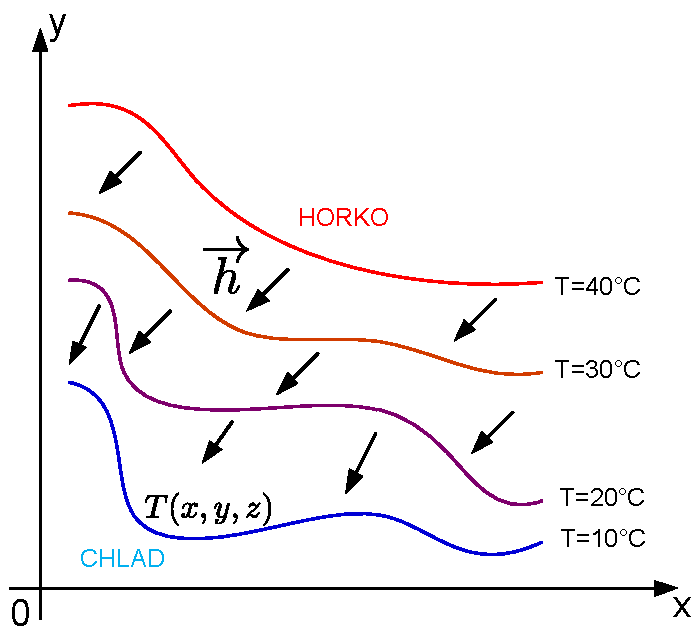
\includegraphics[width=0.5\linewidth]{fyz_fig152_ver1.pdf}
       \caption{Teplota je příkladem skalárního pole. Každému bodu $(x,y,z)$ v prostoru je 
                přiřazeno číslo $T(x,y,z)$. Všechny body na ploše označené $T = 20°C$ (zobrazené 
                jako křivka při $z=0$) mají stejnou teplotu. Šipky jsou ukázkami hustoty tepelného 
                toku $\vec{h}$.
                \cite[s.~29]{Feynman02}}
       \label{fyz:fig152} 
      \end{figure}
            
      U \textbf{vektorových polí} je v každém bodě prostoru dán vektor, který se mění od bodu k
      bodu. Jako příklad vezměme rotující těleso (obr. \ref{fyz:fig032}). Rychlost látky, tvořící
      těleso je v každém bodě vektor, který je funkcí polohy. V druhém případě uvažujme proudění
      tepla z teplejších míst do chladnějších. V různých částech uvažovaného tělesa bude teplo
      proudit různými směry. \emph{Hustota tepelného toku} je veličina, která se vyznačuje směrem.
      Označme ji $\vec{h}$. Její velikost je mírou proudícího tepla. Vektor hustoty tepelného toku
      je vyznačen pro několik poloh i na obr. \ref{fyz:fig152}. Definujeme $\vec{h}$ přesněji.
      Velikost vektoru hustoty tepelného toku udává tepelnou energii, která projde infinitezimálním
      plošným elementem postaveným kolmo na směr toku za jednotku času přepočtenou na  jednotku
      plochy. Vektor má směr toku (obr. \ref{fyz:fig153a}). Vyjádříme to v symbolech: je-li $\Delta
      P$ tepelná energie, která projde za jednotku času
      \begin{equation*}     % \label{temp:eq_tepelny_tok}
       \vec{h}=\frac{\Delta P}{\Delta S}\vec{e_t}
               \quad \vec{e_t}\ldots\text{jednotkový vektor ve směru toku}
      \end{equation*}   

      \luagraphic[0.7]{fyz_fig032.pdf}{Rychlost v rotujícím tělese je příkladem vektorového pole.
      \cite[s.~30]{Feynman02}}{fyz:fig032}
           
      Vektor $\vec{h}$ je možno definovat i jiným způsobem - pomocí jeho složek. Ptejme se, kolik 
      tepla projde malou ploškou postavenou pod libovolným úhlem vzhledem k toku. Obrázek 
      \ref{fyz:fig153b} znázorňuje plošku $\Delta S_2$ skloněnou pod úhlem $\Theta$ k plošce 
      $\Delta S_1$ kolmé na tok. Jednotkový vektor $\vec{n}$ je kolmý na plošku $\Delta S_2$. 
      Vektory $\vec{n}$ a $\vec{h}$ svírají úhel $\Theta$ (neboť $\vec{h}$ je kolmé $\Delta 
      S_1$). Jaká je nyní hustota tepelného toku ploškou $\Delta S_2$? Tok ploškou $\Delta S_2$ je 
      stejný jako ploškou $\Delta S_1$, pouze velikosti obou plošek jsou odlišné, a to $\Delta 
      S_1=\Delta S_2\cos\Theta$. Hustota toku ploškou $\Delta S_2$ je 
      \begin{equation}\label{fyz:eq248}
       \frac{\Delta P}{\Delta S_2}=\frac{\Delta P}{\Delta S_1}\cos{\Theta}=\vec{h}\cdot\vec{n}
      \end{equation}

      \begin{figure}[ht!]
        \centering
        \subcaptionbox{\label{fyz:fig153a}}{\luafigure[0.7]{fyz_fig153a_ver1.pdf}} \newline                                          
        \subcaptionbox{\label{fyz:fig153b}}{\luafigure[0.5]{fyz_fig153b_ver1.pdf}}
        \caption{a) Vektor hustota tepelného toku $\vec{h}$ ukazuje směr proudění. Jeho velikost
                 je rovna energii, která za jednotku času projde elementární ploškou postavenou 
                 kolmo na směr proudění, vydělené obsahem této plošky. b) Tepelný tok ploškou 
                 $\Delta S_2$ je stejný jako tepelný tok ploškou $\Delta S_1$.
                 \cite[s.~30]{Feynman02}}
        \label{fyz:fig153}
      \end{figure}
      
      Tuto rovnici interpretuje tak, že hustotu tepelného toku $\vec{h}$ (teplo prošlé za jednotku 
      času jednotkovou plochou) libovolnou elementární ploškou, jejíž jednotkový normálový vektor 
      je $\vec{n}$, udává výraz $\vec{h}\cdot\vec{n}$. Taktéž bychom mohli říci: složka hustoty 
      tepelného toku kolmá na elementární plošku $\Delta S_2$ je $\vec{h}\cdot\vec{n}$. Chceme-li, 
      můžeme považovat tyto výro\-ky za definice $\vec{h}$. Stejné představy můžeme použít i pro 
      jiná vektorová pole.
        
  % ------------------------ Derivace polí - gradient ----------------------------------------------
  \section{Derivace polí - gradient}
    Mění-li se pole s časem, je možné udávat tyto změny pomocí jejich derivace podle času. Podobným 
    způsobem chceme popsat jejich změny v závislosti na poloze, protože se, řekněme, zajímáme o 
    vztah teploty v jednom místě k teplotě v sousedním místě. Jak vypočteme derivaci teploty podle 
    polohy? Máme derivovat podle $x$? Nebo podle $y$, nebo $z$?
  
    Užitečné fyzikální zákony nezávisí na orientaci souřadnicové soustavy. Proto se musí zapisovat 
    ve tvaru, v němž jsou obě strany buď skaláry, nebo vektory. Co je derivace skalárního pole, 
    například $\pder{T}{x}$. Je to skalár nebo něco jiného? Můžeme se snadno přesvědčit, že to není 
    ani skalár ani vektor, neboť vezmeme-li jinou osu $x$, $\pder{T}{x}$ se jistě změní. Ale 
    všimněme si, že máme tři možné derivace: $\pder{T}{x},\,\pder{T}{y},\,\pder{T}{z}$. Protože 
    existují tři derivace a víme, že tři čísla tvoří vektor, tyto tři derivace by mohly 
    představovat složky jednoho vektoru:
    \begin{equation}\label{fyz:eq249}
      \left(\pder{T}{x},\,\pder{T}{y},\,\pder{T}{z}\right)\overset{?}{=}\mathrm{vektor}
    \end{equation}
    Samozřejmě, ne každá tři čísla obecně tvoří vektor. Je tomu tak pouze tehdy, když při pootočení
    souřadnicové soustavy se složky vektoru správně transformují. Proto je nevyhnutelné prozkoumat, 
    jak se naše tři derivace změní při otočení souřadnicové soustavy. Ukážeme, že rov.     
    \ref{fyz:eq249} je skutečně vektorem. Při otáčení souřadnicové soustavy se derivace    
    transformují správně.
  
    Můžeme se o tom přesvědčit několika způsoby. Jeden způsob je položit si takovou otázku, na níž 
    lze odpovědět nezávisle na souřadnicové soustavě, a pokusit se vy\-já\-dřit odpověď v 
    "invariantním" tvaru. Například jsou-li $\vec{A}$ a  $\vec{B}$ vektory a 
    $S=\vec{A}\cdot\vec{B}$, víme, že $S$ je skalárem. I bez zjišťování \emph{víme}, zda se $S$ 
    mění se změnou souřadnicových soustav. \emph{Nemůže}, neboť jde o skalární součin dvou vektorů. 
    Podobně, \emph{víme-li}, že \(\vec{A}\) je vektorem a mám tři čísla \(B_1\), \(B_2\) a \(B_3\), 
    o kterých zjistíme že
    \begin{equation}\label{fyz:eq250}
      A_xB_1+A_yB_2+A_zB_3=S
    \end{equation}
    kde \(S\) je totéž pro libovolnou souřadnicovou soustavu, pak tři čísla $B_1$, $B_2$ a $B_3$ 
    jsou nutně složkami $B_x$, $B_y$ a $B_z$  nějakého vektoru $\vec{B}$.
  
    Zvažme případ teplotního pole. Vez\-mě\-me dva body $P_1$ a $P_2$ v malé vzdálenosti 
    $\Delta\vec{r}$ od sebe. Teplota v $P_1$ je $T_1$ a v $P_2$ je $T_2$ s rozdílem $\Delta 
    T=T_2-T_1$. Teploty v těchto reálných, fyzikálních bodech určitě nezávisí na volbě os 
    souřadnic. Konkrétně $\Delta T$ je číslo nezávislé na souřadnicové soustavě. Je to skalár.

    \begin{figure}[ht!]  %\ref{fyz:fig031}
      \centering
      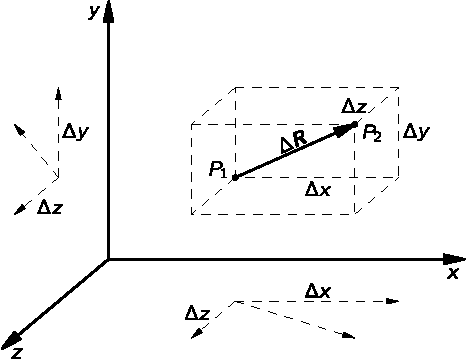
\includegraphics[width=0.6\linewidth]{fyz_fig031_ver1.pdf}
      \caption{Vektor $\vec{r}$, jehož složky jsou $\Delta x,\,\Delta y,\,\Delta z$.}
      \label{fyz:fig031}
    \end{figure}
    Zvolíme-li nějakou vhodnou soustavu souřadnicových os, můžeme napsat $T_1=T(x,y,z)$ a 
    $T_2=T(x+\Delta x,\,y+\Delta y,\,z+\Delta z)$, kde $\Delta x,\,\Delta y,\,\Delta z$ jsou složky 
    vektoru $\Delta \vec{r}$ (obr. \ref{fyz:fig031}). Vzhledem k rovnosti rov. 
    \ref{fyz:eq245} můžeme psát    
    \begin{equation}\label{fyz:eq251}
      \Delta T = \pder{T}{x}\Delta x + \pder{T}{y}\Delta y + \pder{T}{z}\Delta z
    \end{equation}
    Levá strana rovnosti (\ref{fyz:eq251}) je skalárem. Pravá je součtem tří součinů obsahujících 
    jako součinitele $\Delta x,\,\Delta y,\,\Delta z$, které jsou složkami vektoru. Z toho vyplývá, 
    že tři čísla \(\frac{\partial T}{\partial x},\,\frac{\partial T}{\partial y},\,\frac{\partial 
    T}{\partial z}\) Představují také \(x\)-ovou, \(y\)-ovou a \(z\)-ovou složku nějakého vektoru. 
    Pro tento nový vektor použijeme symbol \(\nabla T\). Symbol \(\nabla\) (nazývaný \uv{nabla}) je 
    převráceným \(\Delta\) a má připomínat derivování. \(\nabla T\) se čte různě: \emph{\uv{nabla 
    T}} nebo \emph{\uv{gradient T}} nebo \emph{\uv{grad T}};
    \begin{equation}\label{fyz:eq252}
      \mathrm{grad}\,T =\nabla T = \left(\pder{T}{x},\, \pder{T}{y},\,\pder{T}{z} \right)
      \footnotemark
    \end{equation}
    \footnotetext{V naší symbolice představuje výraz \((a, b, c)\) vektor se složkami \(a\), \(b\),
    \(c\). Použijeme-li jednotkové vektory $\vec{i},\,\vec{j},\,\vec{k}$, můžeme psát
    $$\mathrm{grad}\,T=\nabla T = \vec{i}\pder{T}{x} + \vec{j}\pder{T}{y} + \vec{k}\pder{T}{z}$$}
    Použitím této nové symboliky se můžeme pokusit rovnost (\ref{fyz:eq251}) 
    přepsat na kompaktnější tvar
    \begin{equation}\label{fyz:eq257}
      \Delta T = \nabla T \cdot\Delta\vec{r}
    \end{equation}        

    \begin{figure}[ht!]
      \centering
      \subcaptionbox{\label{fyz:fig154a}}{\luafigure[0.45]{fyz_fig154a_ver1.pdf}}
      \subcaptionbox{\label{fyz:fig154b}}{\luafigure[0.45]{fyz_fig154b_ver1.pdf}}
      \caption{Užitečné fyzikální zákony nezávisí na orientaci souřadnicové soustavy. Dokažme to!
               a) Transformace do pootočené souřadnicové soustavy; b) Speciální případ, v němž je 
               vektor \(\vec{r}\) rovnoběžný s osou \(x\).
               \cite[s.~33]{Feynman02}}
      \label{fyz:fig154}
    \end{figure}

    Tento vztah, vyjádřený slovy, říká, že rozdíl teplot ve dvou sousedních bodech je roven 
    skalárnímu součinu gradientu $T$ a rozdílu polohových vektorů obou bodů. Tvar rov. 
    \ref{fyz:eq257} také ilustruje již uvedený důkaz, že  $\nabla T$ je opravdu vektorem.

    Stále ještě nejste přesvědčeni? Ukážeme, že složky $\nabla T$ se transformují stejně jako 
    složky $\vec{r}$. Pokud ano, $\nabla T$ je vektor podle naší původní definice vektoru. Abychom 
    si to trochu zjednodušili, položme $z=z'$, takže souřadnici $z$ již nemusíme brát v úvahu.

    Uvažujme o soustavě $x'$, $y'$ pootočené o úhel $\Theta$  vzhledem k soustavě $xy$ (obr.
    \ref{fyz:fig154}). Souřadnice bodu $(x,y)$ vyjádřené v čárkované soustavě jsou
    \begin{alignat*}{3}
      x' &=  &&x\cos\Theta &&+ y\sin\Theta             \\
      y' &= -&&x\sin\Theta &&+ y\cos\Theta,            
    \end{alignat*}
    vyjádříme-li $x$ a $y$
    \begin{alignat}{3}
      x  &= &&x'\cos\Theta &&- y'\sin\Theta    \label{fyz:eq253}\\
      y  &= &&x'\sin\Theta &&+ y'\cos\Theta.  \nonumber
    \end{alignat}
    Transformují-li se nějaká dvojice čísel podle těchto rovnic stejně jako $x$ a $y$, jde o složky
    vektoru.

    Nyní si všimněme rozdílu teplot ve dvou sousedních bodech $P_1$ a $P_2$, zvolených tak, jak to
    znázorňuje obr. \ref{fyz:fig154b}. Při výpočtu v souřadnicích $x$ a $y$ můžeme psát
    \begin{align}
      \Delta T  &= \pder{T}{x}\Delta x \quad
                   \text{neboť} \quad \Delta y=0.   \label{fyz:eq254} \\ 
      \shortintertext{A výpočet v čárkované soustavě? Tam bychom psali}
      \Delta T  &= \pder{T}{x'}\Delta x' +
                   \pder{T}{y'}\Delta y'      \label{fyz:eq255}   \\
      \shortintertext{Podíváme-li se na obr. \ref{fyz:fig154b}, vidíme, že}
      \Delta x' &=  \Delta x\cos\Theta \quad \Delta y' = -\Delta x\sin\Theta
    \end{align}
    neboť $\Delta y'$ je záporné při kladném $\Delta x$. Dosazením těchto výrazů do rov.    
    \ref{fyz:eq255} dostaneme
    \begin{align}
      \Delta T    &=  \pder{T}{x'}\Delta x\cos\Theta
                     -\pder{T}{y'}\Delta x\sin\Theta 
                   =  \left(\pder{T}{x'}\cos\Theta   -
                      \pder{T}{x'}\sin\Theta\right)\Delta x  \label{fyz:eq256} \\
      \shortintertext{Porovnáním rov. \ref{fyz:eq256} s rov.   
                      \ref{fyz:eq254} zjistíme, že}
      \pder{T}{x} &=  \pder{T}{x'}\cos\Theta - \pder{T}{y'}\sin\Theta. \label{temp:eq_pT_px}
    \end{align}
    Podle tohoto vztahu $\pder{T}{x}$ dostaneme z $\pder{T}{x'}$ a $\pder{T}{y'}$ právě tak jako 
    $x$ z $x'$ a $y'$ (rov. \ref{fyz:eq253}). $\pder{T}{x}$ je tedy $x-\text{ovou}$ složkou 
    vektoru. Podobné úvahy by ukázaly, že $\frac{\partial T}{\partial y}$ je $y-\text{ová}$ a 
    $\pder{T}{z}$ jeho $z-\text{ová}$ složka. $\nabla T$ je zajisté vektorem. Jde o vektorové pole 
    odvozené ze skalárního pole $T$.
       
  % ------------------------ Operátor nabla ------------------------------------------------------- 
  \section{Operátor \texorpdfstring{\fontsize{16pt}{17pt}\selectfont\(\nabla\)}{nabla}}
    Důkaz, že $\grad{T}$ nebo $\nabla T$ je vektorem, nezávisí na tom, jaké skalární pole jsme 
    derivovali. Všechny úvahy by byly stejné i tehdy, kdyby se $T$ zaměnilo za jakékoliv jiné 
    skalární pole. Transformační rovnice jsou stejné bez ohledu na to, co derivujeme, mohli bychom 
    $T$ vynechat a nahradit rovnici (\ref{temp:eq_pT_px}) operátorovou rovnicí
    \begin{equation}\label{temp:eq_operatorova_rce}
      \pder{ }{x}=\pder{ }{x'}\cos\Theta - \pder{ }{y'}\sin\Theta.
    \end{equation}
    Ponecháme přitom operátory "hladové po derivování".

    Protože diferenciální operátory samotné se transformují stejně jako složky vektoru, můžeme jej 
    nazvat složkami \emph{vektorového operátoru}. Můžeme psát
    \begin{align}
      \nabla   &= \left(\pder{ }{x},\,\pder{ }{y},\,\pder{ }{z}\right)       \label{fyz:eq258}\\
      \shortintertext{což samozřejmě znamená, že}
      \nabla_x &= \pder{ }{x},\quad \nabla_y=\pder{ }{y},\quad\nabla_z=\pder{ }{z}.
    \end{align}  
    Gradient jsme abstrahovali od \(T\).

    Musíme si uvědomit, že operátorová algebra je trochu odlišná od vektorové algebry. S operátory 
    vždy musíme dodržovat správné pořadí, aby operace s nimi měly ten pravý smysl. Co se má 
    derivovat, musí se umístit napravo od $\nabla$. $T\nabla$ je stále operátorem, zatímco $\nabla 
    T$ už není "hladovým" operátorem, neboť se nasytil. Je to opravdový fyzikální vektor, 
    představující rychlost změny $T$ v prostoru. Víme, že rychlost změny $T$ v nějakém směru udává 
    složka vektoru $\nabla T$ v tomto směru (viz vztah \ref{fyz:eq257}). Z toho vyplývá, že 
    $\nabla T$ směřuje tam, kde má největší možnou složku - jinými slovy, směrem, v němž se $T$ 
    mění nejrychleji. \textbf{Gradient $T$ má směr nej\-rychlejšího zvětšo\-vání veličiny $T$.}
    
    % ---------------------- Operace s nabla -------------------------------------------------------
    \subsection{Operace s \texorpdfstring{\(\nabla\)}{nabla}}
      Je možné s vektorovým operátorem $\nabla$ provádět nějaké jiné algebraické operace? Pokusme 
      se kombinovat jej s nějakým vektorem. Dva vektory se kombinují vy\-já\-dře\-ním skalárního 
      součinu. Mohly bychom vytvořit dva součiny
      \begin{equation}\label{fyz:eq259}
        (\mathrm{vektor})\cdot\nabla\quad\mathrm{nebo}\quad\nabla\cdot(\mathrm{vektor})
      \end{equation}
      První součin zatím neznamená nic, protože je to stále pouhý operátor. Jeho konečný smysl by 
      závisel na tom, na co se má aplikovat. Druhý součin je jakési skalární pole. 
      ($(\vec{A}\cdot\vec{B})$ je vždy skalárem.)

      Prozkoumejme skalární součin operátoru $\nabla$ s vektorovým polem, které známe, např. 
      $\vec{h}$.  Vypíšeme-li ho ve složkách
      \begin{align}
        \ndiver{h} &= \nabla_x\cdot h_x +
                      \nabla_y\cdot h_y +
                      \nabla_z\cdot h_z               \label{fyz:eq260}     \\
        \shortintertext{nebo}
        \ndiver{h} &= \pder{h_x}{x} +
                      \pder{h_y}{y} +
                      \pder{h_z}{z}                   \label{fyz:eq261}
      \end{align}
      Tento součet je invariantní vzhledem k transformaci souřadnic. Kdybychom zvolili jinou 
      souřadnicovou soustavu (označenou čárkami), dostali bychom\footnote{Na $\vec{h}$ se díváme 
      jako na fyzikální veličinu, která závisí na poloze v prostoru, a ne, přesně vzato, jako na 
      matematickou funkci tří proměnných. Když je $\vec{h}$ "derivováno" podle $x$,$y$ a $z$ nebo 
      podle $x'$ ,$y'$ a $z'$, je třeba nejdříve vyjádřit matematický výraz pro $\vec{h}$ jako 
      funkci příslušných proměnných. Proto v této nové souřadnicové soustavě neoznačujeme $\vec{h}$ 
      čárkou.}
      \begin{equation}\label{fyz:eq262}
        \nabla'\cdot\vec{h}=\pder{h_{x'}}{x'}+\pder{h_{y'}}{y'}+\pder{h_{z'}}{z'}
      \end{equation}
      což je totéž číslo, které bychom dostali z (rov. \ref{fyz:eq261}), přestože 
      tento vztah vypadá jinak. To znamená, že
      \begin{equation}\label{fyz:eq263}
         \nabla'\cdot\vec{h}= \ndiver{h}
      \end{equation}
      pro každý bod prostoru. Tedy $\nabla\cdot\vec{h}$ je skalární pole, které musí reprezentovat 
      nějakou fyzikální veličinu. Musíte si uvědomit, že kombinace derivací $\nabla\cdot\vec{h}$ je 
      dost specifická.  Existují rozmanité kombinace, např. $\pder{h_y}{x}$, které nejsou ani 
      skaláry, ani složkami vektorů.

      Skalární veličina $\nabla\cdot(\text{vektor})$ je ve fyzice neobyčejně užitečná. Byla nazvána
      \textbf{divergencí} ($\diver{h}$). Například
      \begin{equation}\label{fyz:eq264}
        \ndiver{h}= \diver{h}=\text{divergence}\, \vec{h}.
      \end{equation}
      Podobně jako v případě $\nabla T$ můžeme najít fyzikální význam i pro $\nabla\cdot\vec{h}$.
      Odložíme to však na později.

      Nejdříve se chceme podívat, co můžeme ještě vymyslet pomocí vektorového operátoru $\nabla$. 
      Jak je to s jeho vektorovým součinem? Je třeba očekávat, že
      \begin{equation}\label{fyz:eq265}
        \nrot{h} = \text{vektor}
      \end{equation}
      Složky tohoto vektoru můžeme rozepsat podle obyčejného pravidla pro vektorové součiny (viz 
      rov. \ref{fyz:eq690}).
      \begin{align*}
        (\nrot{h})_x &= \nabla_yh_z-\nabla_zh_y = \pder{h_z}{y} - \pder{h_y}{z} \\
        (\nrot{h})_y &= \nabla_zh_x-\nabla_xh_z = \pder{h_x}{z} - \pder{h_z}{x} \\
        (\nrot{h})_z &= \nabla_xh_y-\nabla_yh_x = \pder{h_y}{x} - \pder{h_x}{y}
      \end{align*}

      Kombinace $\nabla\times\vec{h}$ se nazývá \textbf{rotace} $\vec{h}$ 
      ($\mathrm{rot}\,\vec{h}$). O příčině tohoto pojmenování a o fyzikálním významu této kombinace 
      pojednáme později.

      Celkově tedy máme tři různé kombinace, v nichž vystupuje operátor $\nabla$:
      \begin{equation*}
        \ngrad{T}  =\grad{T}   = \text{vektor} \quad    
        \ndiver{h} =\diver{h}  = \text{skalár} \quad  
        \nrot{h}   =\rot{h}    = \text{vektor}
      \end{equation*}
      Pomocí těchto kombinací můžeme popsat prostorové změny polí ve vhodném tvaru, tj. obecném 
      tvaru, nezávislém na nějaké souřadnicové soustavě.

      Jako příklad použití našeho vektorového diferenciálního operátoru $\nabla$ napíšeme soustavu
      vektorových rovnic obsahujících tytéž zákony elektromagnetizmu - Maxwellovy rovnice:
      \begin{equation}\label{fyz:eq266}
        \begin{array}{c @{{}={}} l r @{{}={}} l}
          \ndiver{E} & \dfrac{\rho}{\varepsilon_0}& \ndiver{B}   & 0,                            \\
          \nrot{E}   & -\pder{\vec{B}}{t}   \quad\quad\quad   & c^2\nabla\times\vec{B} & 
          \pder{\vec{E}}{t} + \frac{\vec{j}}{\varepsilon_0}  
        \end{array}
      \end{equation}

      kde $\rho$ (ró) je hustota elektrického náboje, tj. množství náboje v jednotce objemu, 
      $\vec{j}$ je hustota elektrického proudu, tj. množství náboje, které proteče jednotkovou 
      plochou za sekundu. Tyto čtyři rovnice obsahují úplnou klasickou teorii elektromagnetického 
      pole. Vidíte, jakého elegantního a jednoduchého zápisu můžeme dosáhnout pomocí naší nové 
      symboliky.
      
  % -------- Diferenciální rovnice proudění tepla --------------------------------------------------
  \section{Diferenciální rovnice proudění tepla}
    Uveďme jiný příklad fyzikálního zákona napsaného ve vektorové symbolice. Není to obecně platný 
    zákon, ale pro mnohé kovy a mnoho dalších látek, jež jsou vodiči tepla, je dost přesný. 
    Vezmeme-li kus materiálu v podobě desky a jeho čelní stěnu zahřejeme na teplotu $T_2$, zatímco 
    protilehlou stranu ochladíme na odlišnou teplotu $T_1$, materiálem bude proudit teplo ve směru 
    od $T_2$ k $T_1$ (obr. \ref{fyz:fig155}).
    
    Tepelný tok je přímo úměrný plošnému obsahu $S$ stěn i rozdílu teplot $T_2-T_1$ a nepřímo 
    úměrný vzdálenosti $d$ mezi stěnami. (Pro daný rozdíl teplot platí, že čím tenčí je deska, tím 
    větší je tepelný tok). Nechť $P$ je tepelná energie, která projde deskou za jednotku času. 
    Potom můžeme napsat
    \begin{equation}\label{fyz:eq684}
      \Delta P=\lambda(T_2-T_1)\frac{S}{d},
    \end{equation}
    Konstanta úměrnosti $\lambda$ (lambda) se nazývá \emph{součinitel teplotní vodivosti}.
    
    Co se stane ve složitějším případě, řekněme v tělese nepravidelném tvaru, v jehož objemu se 
    teplota různě mění? Uvažujme kousíček tělesa a představme si v něm takovou destičku, jaká je 
    nakreslená na obr. \ref{fyz:fig155a}, ale v miniaturním měřítku. Nasměrujeme její čelní 
    stěny rovnoběžně s izotermickými hladinami obr. \ref{fyz:fig155b}, takže pro destičku bude 
    platit rov. \ref{fyz:eq684}.
    
    Je-li plošný obsah čelní stěny destičky $\Delta S$, je tepelný tok
    \begin{equation}\label{fyz:eq683}
      P=\lambda(\Delta T)\frac{\Delta S}{\Delta d}
    \end{equation}
    kde $\Delta d$ je tloušťka destičky. $\dfrac{\Delta P}{\Delta S}$ jsme definovali jako velikost
    vektoru $\vec{h}$ ležícího ve směru tepelného toku. 

    \begin{figure}[ht!]
      \centering
      \subcaptionbox{\label{fyz:fig155a}}{\luafigure[0.4]{fyz_fig155a_ver1.pdf}}
      \subcaptionbox{\label{fyz:fig155b}}{\luafigure[0.4]{fyz_fig155b_ver1.pdf}}
      \caption{a) Tepelný tok deskou. b) Infinitezimální destička rovnoběžná s izotermickou 
               hladinou ve velkém kuse látky \cite[s.~38]{Feynman02}}
      \label{fyz:fig155}
    \end{figure}

    Teplo bude proudit od $T_1+\Delta T_1$ k $T_1$ a tudíž kolmo na izotermy (obr.
    \ref{fyz:fig155b}). $\dfrac{\Delta P}{\Delta d}$ udává dále právě rychlost změny $T$ při změně
    polohy. Protože poloha se mění ve směru kolmém na izotermy, naše $\dfrac{\Delta T}{\Delta d}$
    udává maximální rychlost změny $T$, a tedy velikost vektoru $\nabla T$. Protože směr $\nabla T$
    je opačný než směr\footnote{Záporné znaménko je nutné, neboť teplo proudí ve směru poklesu
    teploty.} $\vec{h}$  rov. \ref{fyz:eq683} zapsaná pomocí vektorů bude vypadá takto
    \begin{equation}\label{fyz:eq685}
      \vec{h}=-\lambda\nabla T
    \end{equation}
    Rovnice \ref{fyz:eq685} je diferenciální rovnicí vedení tepla v masivních 
    tělesech. Jde o skutečnou vektorovou rovnici. Každá její strana je vektor, je-li $\lambda$ jen 
    číslo. Je zobecněním speciální rov. \ref{fyz:eq683} pro pravoúhlé desky na 
    libovolné případy. Tato symbolika je užitečný nejen proto, že v ní rovnice vypadají 
    jednodušeji, ale i proto, že nejjasněji ukazuje fyzikální obsah rovnic bez odvolání na nějakou 
    libovolně zvolenou souřadnicovou soustavu.      
    
  %---------------- Druhé derivace vektorových polí ------------------------------------------------
  \section{Druhé derivace vektorových polí}\label{sec:fey_diff_2deriv}
    Dosud jsme měli pouze první derivace. Proč se však nezabývat i druhými derivacemi? Mohli bychom
    sestavit několik kombinací:
    \begin{enumerate}[leftmargin=2cm,rightmargin=2cm, label=\emph{\alph*}),noitemsep]
      \setlength{\itemsep}{0cm}%
      \setlength{\parskip}{0em}%
      \item $\nabla\cdot(\nabla T)$
      \item $\nabla\times(\nabla T)$
      \item $\nabla\cdot(\ndiver{h})$
      \item $\nabla\cdot(\nrot{h})$
      \item $\nabla\times(\nrot{h})$
    \end{enumerate}
    Můžeme se přesvědčit, že to jsou všechny možné kombinace.
  
    Podívejme se nejdříve na druhou z nich, tj. na b). Má stejný tvar jako 
    $\vec{A}\times(\vec{A}T)= (\vec{A}\times\vec{A})T = 0$, neboť $\vec{A}\times\vec{A}$ je 
    vždy \(0\). Z toho tedy vyplývá, že
    \begin{equation}\label{fyz:eq239}
      \mathrm{rot}\,\grad{T} = \nabla\times\nabla T = 0.
    \end{equation}
    Jak dochází k této rovnosti, můžeme vidět, když si výraz b) napíšeme ve složkách: 
    \begin{align*}
      [\nabla\times(\nabla T)]_z 
          &= \nabla_x(\nabla T)_y-\nabla_y(\nabla T)_x                                   \\
          &= \pder{}{x}\left(\pder{T}{y}\right) - \pder{}{y}\left(\pder{T}{x}\right)
    \end{align*}
    což je nula podle rovnosti (\ref{fyz:eq246}). Stejně je to pro další složky.
    \(\nabla\times(\nabla T)=0\) tedy platí pro jakékoliv rozdělení teploty - dokonce pro 
    \emph{jakoukoliv} skalární funkci.
  
    Vezměme si jiný příklad. Podívejme se, zda se nám podaří dostat i jiný výraz rovný nule. 
    Skalární součin vektoru s vektorovým součinem obsahující tentýž vektor dává nulu
    \begin{equation*}
      \vec{A}\cdot(\vec{A}\times\vec{B}) = 0
    \end{equation*}
    neboť \((\vec{A}\times\vec{B})\) je kolmé na \(\vec{A}\) a jeho složka ve směru \(\vec{A}\) je 
    tedy nulová. Stejná kombinace se vyskytuje v rovnici d), a tak dostáváme
    \begin{equation}\label{fyz:eq686}
      \nabla\cdot(\nabla\times\vec{h}) = \mathrm{div}\,(\rot{h})= 0.
    \end{equation}
    Snadno se opět ukáže, že je to \(0\), zapíší-li se naznačené operace ve složkách.
  
    Nyní zformulujeme dvě matematické věty, které nebudeme dokazovat. Jsou to velice zajímavé věty 
    a je pro fyziky užitečné je znát. 
  
    Ve fyzikálních úlohách často zjistíme, že rotace nějaké veličiny, řekněme vektorového pole 
    \(\vec{A}\), je nula. Viděli jsme (rovnost \ref{fyz:eq239}), že rotace gradientu je rovna 
    nule, což se vzhledem k vlastnostem vektorů dobře pamatuje. Bylo by tedy dobře možné, aby bylo 
    \(\vec{A}\) gradientem nějaké veličiny; jeho rotace by pak byla nutně nulová. Platí zajímavá 
    věta, podle které, je-li \(\rot{A}\) rovna nule, je \(\vec{A}\) vždy gradientem něčeho, a tedy 
    existuje určité skalární pole \(\Psi\) (psí) takové, že \(\vec{A}\) je rovno \(\grad{\Psi}\) 
    Jinými slovy platí následující věta
    \begin{lemma}
      Je-li $\nabla\times\vec{A}=0$, existuje $\psi$ takové, že $\vec{A} = \nabla\psi$
    \end{lemma}
    Podobná věta platí i v případě, že div A je rovna nule. Rovnost (\ref{fyz:eq686}) říká, že
    divergence rotace něčeho je vždy nula. Setkáme-li se s vektorovým polem \(\vec{D}\), přičemž 
    \(\diver{D}\) je rovna nule, můžeme z toho usoudit, že \(\vec{D}\) je rotací nějakého vektorového pole 
    \(\vec{C}\).
    \begin{lemma}
      Je-li $\diver{D} = 0$, existuje $\vec{C}$ takové, že $\vec{D} = \nabla\times\vec{C}$.
    \end{lemma}
    Při zkoumání možných kombinací dvou operátorů \(\nabla\) jsme zjistili, že dvě z nich dávají 
    vždy nulu. Podívejme se nyní na ty, které nejsou nulové. Vezměme kombinaci 
    \(\nabla\cdot(\ngrad{T})\), která byla v našem záznamu napsaná jako první. Obecně nulu nedává. 
    Vypíšeme složky: 
    \begin{align*}
      \ngrad{T}              &= (\nabla_xT, \nabla_yT, \nabla_zT).  \\
      \shortintertext{Potom}
      \nabla\times(\nabla T) &= \nabla_x(\nabla_xT) + \nabla_y(\nabla_yT) + \nabla_z(\nabla_zT)   \\
                             &= \ppder{T}{x} + \ppder{T}{y} + \ppder{T}{z}.
    \end{align*}
    z čehož v obecném případě dostaneme nějaké číslo. Jde o skalární pole. 
  
    Vidíme, že není třeba ani dávat závorky a aniž bychom riskovali záměnu, můžeme psát \(\nabla 
    \cdot(\nabla T) = (\nabla\cdot\nabla)T = \nabla\cdot\nabla T = \nabla^2T\). Na \(\nabla^2\) se 
    díváme jako na nový operátor - \textbf{Laplaceův operátor}:
    \begin{equation}\label{fyz:eq687}
      \text{Laplaceův operátor} = \nabla^2 = \ppder{}{x} + \ppder{}{y} + \ppder{}{z}.
    \end{equation}
    Protože Laplaceův operátor je skalárním operátorem, můžeme jím působit i na vektor - myslíme 
    tím tutéž operaci na každou složku vektoru v pravoúhlé souřadnicové soustavě:
    \begin{equation*}
      \nabla^2\vec{h} = (\nabla^2h_x, \nabla^2h_y, \nabla^2h_z).
    \end{equation*}
    Podívejme se na další možnost, kterou je rovnice e), tj. \(\nabla\times\nabla\times\vec{h}\). 
    Vzhledem k vektorové rovností (\ref{fey:eq_baccab}) můžeme rotaci vyjádřit jinak. Při použití 
    výše této rovnice 
    musíme \(\vec{A}\) a \(\vec{B}\) nahradit operátorem \(\nabla\) a položit \(\vec{C} = \vec{h}\).
    \begin{equation*}
      \nabla\times(\nrot{h}) = \nabla(\nabla\cdot\vec{C}) - \vec{h}(\nabla\cdot\nabla) \ldots ???
    \end{equation*}
    Okamžik! Něco je špatně. První dva členy jsou totiž vektory, jak to má být (operátory v nich 
    jsou „nasycené“), ale poslední člen není v pořádku. Má stále charakter operátoru. Chyba je v 
    tom, že jsme nebyli dost pozorní při dodržování pořadí symbolů v zápisech našich členů. Když si 
    znovu všimneme rovnosti (\ref{fey:eq_baccab}), zjistíme, že bychom ji mohli stejně dobře napsat 
    ve tvaru:
    \begin{align*}
      \vec{A}\times(\vec{B}\times\vec{C}) 
        &= \vec{B}\cdot(\vec{C}\cdot\vec{A}) - (\vec{A}\cdot\vec{B})\cdot\vec{C}  \\
      \shortintertext{Pořadí členů teď vypadá líp. Proveďme substituci do této rovnice. Dostáváme} 
      \nabla\times(\nabla\times\vec{h})
        &= \nabla(\ndiver{h}) - (\nabla\cdot\nabla)\vec{h} 
    \end{align*}
    Tento tvar se zdá být v pořádku. Skutečně je správný, o tom se můžete přesvědčit výpočtem 
    složek. Poslední člen je Laplaceův operátor a tak můžeme stejně dobře napsat
    \begin{equation*}
      \nabla\times(\nabla\times\vec{h}) = \nabla(\ndiver{h}) - \nabla^2\vec{h}.
    \end{equation*}
    Již jsme se zmínili o všech kombinacích v našem seznamu výrazů v úvodu kapitoly  
    \ref{sec:fey_diff_2deriv} s dvojitým operátorem \(\nabla\) s výjimkou případu c), 
    tj.\(\nabla(\nabla\cdot\vec{h})\). To je přípustné vektorové pole, ale nic zvláštního se o něm 
    říci nedá. Jde pouze o určité vektorové pole, které se může příležitostně vyskytnout.

    Bude vhodné, když naše závěry shrneme:
    \begin{mdframed}[style=mdnote]
        \begin{alignat*}{2}
          \nabla\cdot(\nabla T)         &= \nabla^2 T && \ldots\text{skalární pole}   \\
          \nabla\times(\nabla T)        &= 0          &&                               \\
          \nabla\cdot(\ndiver{h})       &= ?           && \ldots\text{vektorové pole}  \\
          \nabla\cdot(\nrot{h})         &= 0          &&                               \\
          \nabla\times(\nrot{h})        &= \nabla(\ndiver{h}) - \nabla^2\vec{h}&&      \\
        (\nabla\cdot\nabla)\cdot\vec{h} &= \nabla^2\vec{h} && \ldots\text{vektorové pole}
        \end{alignat*}
    \end{mdframed}
    Všimněme si, že jsme se nepokusili zavést nový operátor \(\nabla\times\nabla\). Víme proč?
    
  %---------------- Nástrahy -----------------------------------------------------------------------
  \section{Nástrahy}\label{sec:fey_diff_traps}
    \cite[s.~41]{Feynman02} Naši znalost obvyklé vektorové algebry jsme aplikovali na algebru 
    operátoru \(\nabla\). Musíme přitom však být opatrní, neboť se můžeme dostat na scestí. Zmíníme 
    se o dvou nástrahách. V tomto kursu se však nevyskytnou. Co byste řekli následujícímu výrazu, 
    který obsahuje dvě skalární funkce \(\psi\) a \(\varphi\) (fí):
    \begin{align*}
      (\nabla\psi) &\times(\nabla\varphi)? 
      \shortintertext{Asi bychom chtěli prohlásit: musí to být nula, protože je to stejné jako}
      (\vec{A}a)   &\times(\vec{B}b),     
    \end{align*}
    což je rovno nule, neboť vektorový součin dvou stejných vektorů \(\vec{A}\times\vec{A}\) je 
    vždy nula. Ale v našem případě dva operátory \(\nabla\) nejsou stejné. První působí na jednu 
    funkci, a to \(\psi\), zatímco druhý působí na jinou funkci, tj. \(\varphi\). Proto ačkoliv je 
    označujeme tímtéž symbolem  \(\nabla\), je třeba o nich uvažovat jako o odlišných operátorech. 
    Je to pochopitelné, vždyť směr \(\nabla\psi\) závisí na funkci \(\psi\), a proto asi nebude 
    rovnoběžný s \(\nabla\varphi\).
    \begin{equation*}
      (\nabla\psi)\times(\nabla\varphi)\neq0 \text{ (obecně)}. 
    \end{equation*}
    My, naštěstí, nebudeme muset takové výrazy použít. (Co jsme právě řekli, nemění nic na faktu, 
    že \(\nabla\times\nabla(\psi)=0\) pro jakékoli skalární pole, neboť zde působí oba operátory 
    \(\nabla\) na stejnou funkci.)

    Nástraha číslo dvě (které se opět v kurzu vyhneme) spočívá v tomto: Pravidla, která jsme tu 
    uvedli, jsou jednoduchá a pěkná, když se použijí pravoúhlé souřadnice. Máme-li například 
    \(\nabla^2\vec{h}\) a potřebujeme složku \(x\), hned píšeme
    \begin{equation*}
      (\nabla^2\vec{h})_x = \left(\frac{\partial^2}{\partial x^2} + 
                                  \frac{\partial^2}{\partial y^2} + 
                                  \frac{\partial^2}{\partial z^2} 
                            \right)
    \end{equation*}
    Stejný výraz se však nedá napsat, kdybychom se ptali na radiální složku \(\nabla^2\vec{h}\). 
    Radiální složka \(\nabla^2\vec{h}\) není rovna výrazu \((\nabla^2\vec{h})_r\). Příčina je v 
    tom, že máme-li co dělat s vektorovou algebrou, jsou směry všech vektorů plně určeny. Ale pokud 
    jde o vektorová pole, jsou jejich směry v různých místech různé. Pokusíme-li se popsat 
    vektorové pole, řekněme v polárních souřadnicích, to, co nazýváme radiálním směrem, se od bodu 
    k bodu mění. Proto se můžeme dostat do velkých těžkostí, když začneme derivovat složky. 
    Například i pro konstantní vektorové pole se radiální složka bod od bodu mění.

    Obvykle je nejbezpečnější a nejjednodušší držet se pravoúhlých souřadnic a vyhnout se těžkostem.
    Je tu však jedna výjimka, která stojí za zmínku: Protože Laplaceův operátor \(\nabla^2\) je
    skalár, můžeme jej psát v souřadnicové soustavě jaké jen chceme (např. v polárních
    souřadnicích). Ale protože je to diferenciální operátor, smíme jej použít pouze na vektory,
    jejichž složky mají pevný směr, tj. na složky dané v pravoúhlé souřadnicové soustavě. Proto
    budeme-li naše vektorové diferenciální rovnice sát ve složkách, budeme všechna vektorová pole
    vyjadřovat pomocí jejich x-ových, y-ových a z-ových složek.

  \section{Cvičení}
      %---------------------------------------------------------------
      % !TeX spellcheck = cs_CZ
\begin{mdframed}[style=mdexam]
\begin{example}
  Jestliže platí, že \(\rot{A} = \rot{B}\), plyne z toho že \(\vec{A}=\vec{B}\)?\newline  
  \textbf{Řešení:} 
  Nikoliv. Mějme následující funkci \(\vec{A} = \vec{B} + \grad{\varPsi}\), kde 
  \(\varPsi(\vec{r})\) je libovolná skalární funkce (tedy \(\vec{A}\neq\vec{B}\)), pak platí
  \[\rot{A} = \rot{B} +\mathrm{rot}\;\grad{\varPsi} = \rot{B}\] (rotace gradientu je pro 
  spojité funkce vždy nulová, viz \ref{fyz:eq239} kapitola \ref{fyz:IIchapIIsecVII})
\end{example}
\end{mdframed}
      %---------------------------------------------------------------

      %---------------------------------------------------------------
      \begin{fyzexam}{Divergence el. pole bodového náboje}{exam009}
  Nalezněte divergenci elektrického pole bodového náboje v celém prostoru (pro 
  \textbf{bodový náboj} je \(r\rightarrow0\), \(\varrho\rightarrow\infty\)).
  (zdroj: \librariaALDBR)

\tcbsubtitle[before skip=\baselineskip]{Řešení:}  
  Elektrické pole v okolí bodového náboje je dáno \hyperlink{fyz:IIchapIVsecII}{Coulombovým zákonem}
  \[\vec{E} = \frac{Q}{4\cdot\pi\cdot r^2}\vec{n}_0,\] kde \(r\) je vzdálenost daného místa od
  náboje, \(\vec{n}_0\) je jednotkový vektor \(\vec{n}_0 = \left(\dfrac{x}{r}, \dfrac{y}{r},
  \dfrac{z}{r}\right)\) mířící od náboje. Elektrické pole má tedy složky \(\left(k =
  \dfrac{Q}{4\cdot\pi\cdot r^2}\right)\)
  \begin{equation*}
    E_x = k\left(\frac{x}{r^3}\right), \quad
    E_y = k\left(\frac{y}{r^3}\right), \quad
    E_z = k\left(\frac{z}{r^3}\right).
  \end{equation*}
  Pro výpočet divergence budeme potřebovat derivaci vzdálenosti podle jednotlivých
  proměnných:
  \begin{align*}
    \pder{r}{x} &= \pder{(x^2 + y^2 + z^2)^\frac{1}{2}}{x} = \frac{x}{r},  \\
    \pder{r}{y} &= \pder{(x^2 + y^2 + z^2)^\frac{1}{2}}{y} = \frac{y}{r},  \\ 
    \pder{r}{z} &= \pder{(x^2 + y^2 + z^2)^\frac{1}{2}}{z} = \frac{z}{r}.  \\
    \shortintertext{Divergence elektrického pole je, jak známo}            
    \diver{E}   &= \pder{E_x}{x} + \pder{E_y}{y} + \pder{E_z}{z}.
  \end{align*}
  Derivace jednotlivých složek je v tomto případě optimální řešit jako derivace podílu:
  \begin{align*}
    \pder{E_x}{x}  &=  \pder{ }{x}\left(k\dfrac{x}{r^3}\right)         
                    = k\pder{ }{x}\left(\dfrac{x}{r^3}\right)                \\ 
                   &= k\dfrac{\pder{x}{x}r^3-x3r^2\pder{x}{r}}{r^6}          \\
                   &= k\dfrac{r^3-x3r^2\dfrac{x}{r}}{r^6}
                    = k\dfrac{r^2-3x^2}{r^5}
  \end{align*}
  Podobně bude
  \begin{equation*}
    \pder{E_y}{y} = k\dfrac{r^2-3y^2}{r^5} \quad a \quad
    \pder{E_z}{z} = k\dfrac{r^2-3z^2}{r^5},
  \end{equation*}
  takže pro divergenci máme
  \begin{align*}
    \diver{E} &= k\dfrac{r^2 - 3x^2 + r^2 - 3y^2 + r^2 - 3z^2}{r^5}       \\
              &= k\dfrac{3r^2-3(x^2 + y^2 + z^2)}{r^5} = 0; \quad r\neq0
  \end{align*}
  Divergence elektrického pole je tedy v celém prostoru nulová (nejsou v něm zřídla toku) kromě 
  množiny \(r = 0\), ve které se toto zřídlo (zdroj pole - singulární hustota náboje) nachází.
\end{fyzexam}
      %---------------------------------------------------------------
      
      %---------------------------------------------------------------
      % !TeX spellcheck = cs_CZ
\begin{mdframed}[style=mdexam]
\begin{example}
  Nadmořská výška libovolného bodu na povrchu kopce je dána formulí
  \begin{equation*}
    h(x, y) = A\cdot\exp{\left[
                           −\left(\frac{x}{l_0}\right)^2
                          −9\left(\frac{y}{l_0}\right)^2
                         \right]},
  \end{equation*}
  kde \(A = \SI{500}{\m}\), \(l_0 = \SI{100}{\m}\). Nalezněte směr největšího stoupání do kopce 
  (malé posunutí po povrchu kopce v tomto směru vyvolá největší přírůstek nadmořské výšky) v bodě 
  \(B = [-30, 10]\,\si{m}\).
  
  \textbf{Řešení}: Směr největšího stoupání vyjadřuje gradient skalární funkce, kterou je popsána 
  povrchová plocha kopce. Platí
  \begin{align*}
    \vec{n} &= \grad h = \left(\pder{h}{x}, \pder{h}{y}\right)                       \\
            &= \frac{2A}{l_0}\exp{\left[−\left(\frac{x}{l_0}\right)^2
                −9\left(\frac{y}{l_0}\right)^2\right]}(x,9y) \approx (-x,-9y)
  \end{align*}
  Nepodstatné konstanty mění jen délku vektoru, nikoliv jeho směr, proto jsou v konečném  výsledku 
  vynechány. V bodě \(B\) je tedy směr největšího stoupání určen vektorem

  \vspace{0.5cm}
  {\centering
    \captionsetup{type=figure}
    \luafigure[1]{fyz_fig0201.png}
    \captionof{figure}{ }
    \label{fyz:fig0017}
  \par}
  
  \begin{equation*}
   \vec{n}_B \approx (+30, -90) \approx (+10, -30) \approx (+1, -3).
  \end{equation*}
  \begin{itemize}
    \item zdroj: \librariaALDBR
%   \attachfile[icon=Paperclip, description=FYZ000.m]{../SRC/FYZ/matlab/FYZ000.m}
  \end{itemize}  
  %---------------------------------------------------------------
  \lstinputlisting[%
    style=luaMatlabStyle, firstline=7,
    caption={\texttt{FYZ000.m}: Výpis programu pro určení směru největšího stoupání do kopce.}
    ]{../src/FYZ/matlab/FYZ000.m}
  %---------------------------------------------------------------  
\end{example}
\end{mdframed}
      %---------------------------------------------------------------

      %---------------------------------------------------------------
      % !TeX spellcheck = cs_CZ
\begin{fyzexam}{Deskový kondenzátor}{exam013}
  Mějme nabitý deskový kondenzátor \(C\) (obr. \ref{teo:fig013a}). Zvětšíme jeho kapacitu, například
  tím, že zvětšíme plochu jeho elektrod, nebo připojíme paralelně druhý stejné velikosti, viz obr.
  \ref{teo:fig019b}. Otázka zní, jak velká energie bude uložena v elektrostatickém poli obou
  kondeznátorů? Bude energie po rozdělení náboje mezi oba kondenzátory rovna původní energii
  nabitého kondenzátoru? Pokud ne, vysvětlete kam se část energie transformovala. 
  
  {\centering
    \vspace{1em}
    \captionsetup{type=figure, skip=1pt}
    \subcaptionbox{\label{fyz:fig0959a}}{\luafigure[0.15]{fyz_fig0959a.pdf}}           
    \hfill
    \subcaptionbox{\label{fyz:fig0959b}}{\luafigure[0.55]{fyz_fig0959b.pdf}}
    \captionof{figure}{K příkladu \ref{fyz:exam013}: a) Nabitý kondenzátor s rovnoběžnými
    rovinnými elektrodami; b) Rozložení náboje na obou kondenzátorech stejné velikosti.
    }
    \label{fyz:fig0959}
  \par}

\tcbsubtitle[before skip=\baselineskip]{Řešení:}      
  Je-li dielektrikum kondenzátoru lineární, pak pro energii elektrického pole akumulované v
  nabitém kondenzátoru platí. Podrobněji například v kapitole \ref{fyz:IIchapVsecXIX}.
  \begin{equation}
    W = \frac{1}{2}CU^2 \;\text{nebo}\; W = \frac{1}{2}\frac{Q^2}{C} \;\text{kde}\; 
    C = \frac{Q}{U}
  \end{equation}
  Předpokládejme ustálený stav po připojení druhého kondenzátoru, jak je znázorněno na obr.
  \ref{fyz:fig0959b}. V obvodu nepředpokládáme přítomnost odporu, který by způsobil ztrátu energie,
  vyzářené v podobě tepla. Kapacita je dvojnásobná a náboj zůstal stejný. Na každém kondenzátoru
  tedy očekáváme polovinu původního náboje. Sečteme-li energii uloženou v elektrických polích obou
  kondenzátorů dostaneme
  \begin{align*}
    W^* &= \frac{1}{2}\frac{(\frac{1}{2}Q)^2}{C} + \frac{1}{2}\frac{(\frac{1}{2}Q)^2}{C}   \\
        &= \frac{(\frac{1}{2}Q)^2}{C} =\frac{1}{4}\frac{Q^2}{C}                 
          \xrightarrow[C\rightarrow2C]{}
          \frac{1}{2}\frac{Q^2}{(2C)} = \frac{1}{2}W 
  \end{align*}
  Kupodivu, polovina energie prostě chybí a jelikož platí zákon zachování energie\footnote{viz
  partie Fyzika \ref{vol02:part:FYZI}, kapitola \ref{vol02:fyz:IchapIV})}, nezbývá nic jiného než
  uznat, že elektrický obvod dle \ref{fyz:fig0959b}, nemodeluje fyzikální problém dost věrně. Tím
  jsme dospěli k závěru, že je nutné do obvodu dodat rezistor, tak jak je znázorněno na obrázku
  \ref{fyz:fig0960}.
  
  Abychom mohli určit tepelné ztráty na rezistoru dané integrálem \(\int_{0}^{\infty}
  Ri^2(t)\dd{t}\), nejdříve sestavíme jednoduchou diferenciální rovnici prvního řádu aplikací II.
  Kirchhoffova zákona, ze které odvodíme vzorec pro časovou závislost proudu \(i(t) =
  \diff{Q(t)}{t}\). 
  \begin{align*}
    \frac{Q_0 - Q(t)}{C} - Ri(t) - \frac{Q(t)}{C}           &= 0 \quad/\der{ }{t}             \\
    -\frac{i(t)}{C} - R\der{i(t)}{t} - \frac{i(t)}{C} &= 0                              \\
                                        \der{i(t)}{t} &= - \frac{2}{RC}i(t) \quad/\int  \\
                                                  i(t) &= I_0e^{-\frac{2}{RC}t}
  \end{align*}
  
  {\centering
  \captionsetup{type=figure}
  \luafigure[0.6]{fyz_fig0960.pdf}
  \captionof{figure}{Rezistor \(R\) představuje ztráty, které nebyly v obvodu na obrázku 
    \ref{fyz:fig0959} předpokládány} 
  \label{fyz:fig0960}
  \par}

  Nyní můžeme stanovit energii disipované na rezitoru \(R\)
  \begin{align*}
    W   &= \int_{0}^{\infty}Ri^2(t)\dd{t} = RI_0^2\int_{0}^{\infty}e^{-\frac{4}{RC}t}\dd{t}   \\
    \shortintertext{Do integrované funkce dosadíme novou proměnnou \(u = \frac{4}{RC}t\), \(\dd{u} 
                    = \frac{4}{RC}\dd{t}\), \(\dd{t} = \frac{RC}{4}\dd{u}\)}
        &= RI_0^2\int_{0}^{\infty}e^{-u}\frac{RC}{4}\dd{u} 
        = R^2I_0^2\frac{C}{4}\underbrace{\int_{0}^{\infty}e^{-u}\dd{u}}_1 
    \end{align*}
  Jelikož platí \[I_0 = \frac{U}{R}=\frac{Q}{CR}\] dostaneme po dosazení
  \[\cancel{R^2}\frac{Q^2}{C^2\cancel{R^2}}\frac{C}{4} = \frac{Q^2}{4C}= \frac{1}{2}W.\] Nyní je
  vše v pořádku. Druhá polovina energie je disipována na rezistoru a navíc z výsledku vyplývá, že
  vůbec nezávisí na \(R\)!
\end{fyzexam}
      %---------------------------------------------------------------      
%} %tikzset
%~~~~~~~~~~~~~~~~~~~~~~~~~~~~~~~~~~~~~~~~~~~~~~~~~~~~~~~~~~~~~~~~~~~~~~~~~~~~~~~~~~~~~~~~~~~~~~~~~~